\documentclass[aspectratio=169]{beamer}
\usepackage{tikz}
\usepackage{fancyvrb}
\usepackage{xcolor}
\title{Introduction to Reversing with Z3\\RPISEC}
\date{December 3, 2019}
\author{Avi Weinstock (\Verb|aweinstock|)}

\definecolor{rpisecbgcolor}{RGB}{21, 24, 32} % 151820
\definecolor{cybercyan}{RGB}{42, 171, 219} % 2aabdb
\definecolor{cybergreen}{RGB}{106, 220, 169} % 6adca9
\definecolor{cyberpink}{RGB}{248, 106, 140} % f86a8c

\setbeamercolor{normal text}{fg=white}
\setbeamercolor{frametitle}{fg=cybercyan}
\setbeamercolor{title}{fg=cybercyan}
\setbeamercolor{structure}{fg=cybercyan}

%>>> [0x15,0x18,0x20]
%[21, 24, 32]
% convert rpisec_background.png -alpha set -fill '#15182080' -draw 'rectangle 0 0 1090 1216' rpisec_background2.png
% convert probable_prime.png -alpha set -fill '#151820c0' -draw 'rectangle 0 0 414 836' probable_prime2.png
\usebackgroundtemplate{
\colorbox{rpisecbgcolor}{\raisebox{1pt}[\paperheight][\depth]{\hspace{0.6\paperwidth}
%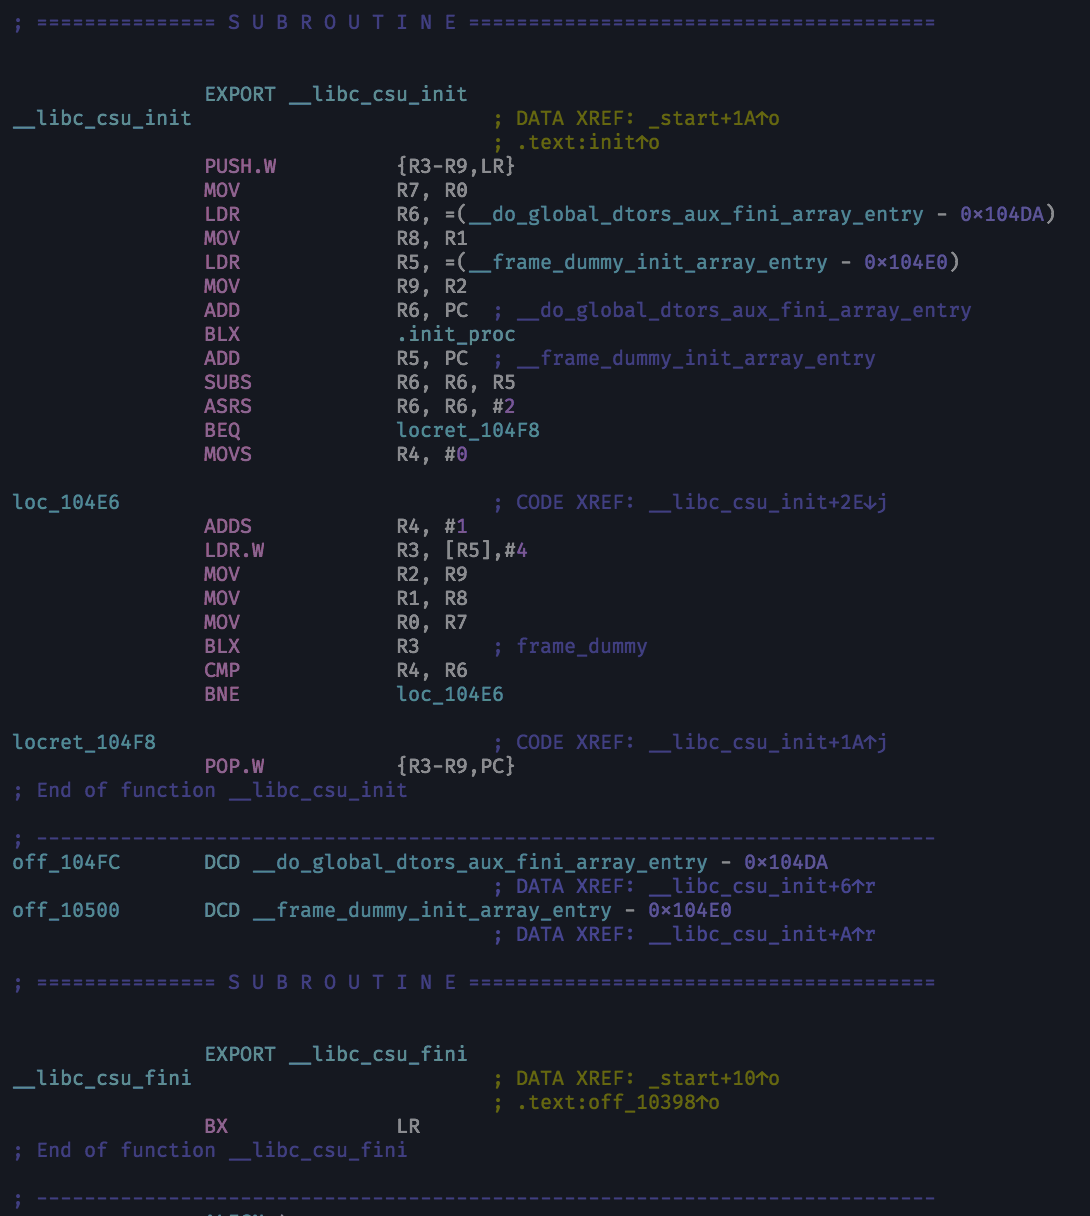
\includegraphics[width=0.4\paperwidth, height=\paperheight]{rpisec_background2.png}
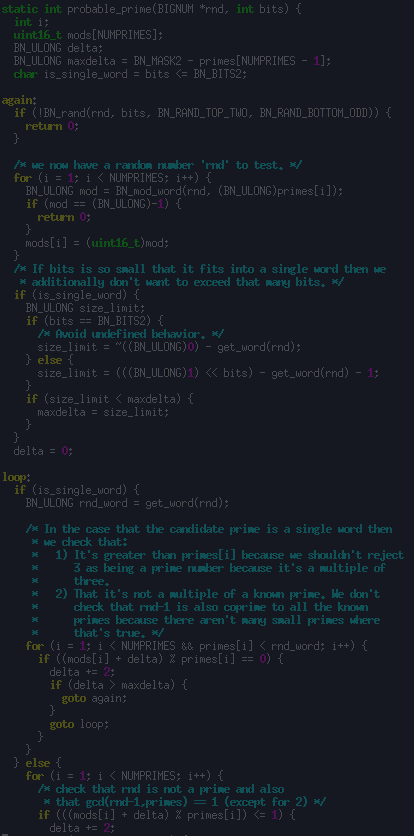
\includegraphics[width=0.4\paperwidth, height=\paperheight]{../rsa_2019_10_29/probable_prime2.png}
}}
}

\begin{document}
\maketitle

\begin{frame}[fragile]
\frametitle{Overview}
\begin{itemize}
\item What are SAT/SMT/Z3?
\item Solving MBE lab1A with Z3
\item Solving a Cyberseed RE challenge with Z3
\end{itemize}
\end{frame}

\begin{frame}[fragile]
\frametitle{What is SAT?}
\begin{itemize}
\item SAT is the boolean SATisfiability problem
\item e.g. "Does the formula $(x \lor \neg y \lor z) \land (\neg x \lor y)$ have a satisfying assignment?"
\begin{itemize}
\item $(\neg, \land, \lor)$ mean (NOT, AND, OR)
\end{itemize}
\item Brute forceable in $O(2^n)$ by trying all combinations of $\{0,1\}$ for all variables
\item NP-Complete 
\begin{itemize}
\item \textcolor{red}{Con:} Impossible\footnote{Unless P=NP} to solve quickly\footnote{In polynomial time}
\item \textcolor{green}{Pro:} Many problems can be expressed as SAT instances, so heuristics for SAT can help solve many problems
\end{itemize}
\end{itemize}
\end{frame}

\begin{frame}[fragile]
\frametitle{What is SMT?}
\begin{itemize}
\item SMT is Satisfiability Modulo Theories
\item "Does $(f(x,y) \lor z) \land (\neg g(x) = f(x, x))$ have a satisfying assignment?" (QF-EUF)
\item "Does $(2*x+y \le z) \land (x+3*y \ge z)$ have a satisfying assignment" (QF-LIA)
\item Allows more compact translation of problems, e.g.
\begin{itemize}
\item $x = 1 \lor x = 2 \lor x = 3 \lor \hdots \lor x = 99 \lor x = 100$ (SAT)
\item $1 \le x \land x \le 100$ (SMT)
\end{itemize}
\item Also NP-Complete
\end{itemize}
\end{frame}

\begin{frame}[fragile]
\frametitle{Why are SAT/SMT useful if they're hard to solve quickly?}
\begin{itemize}
\item Not all problems are as hard as the hardest ones
\begin{itemize}
\item 2-SAT (each clause having at most 2 variables) is polytime solvable
\item Monotone circuits (only ANDs and ORs, no NOTs) are polytime solvable
\end{itemize}
\item It's often possible to prune the search space 
\begin{itemize}
\item e.g. $x \lor \varphi(a, b, c, \hdots)$ is solvable regardless of $\varphi$ because $x=1$ cancels out that subterm
\end{itemize}
\item Algorithms like DPLL and CDCL make use of partial structure to solve some instances faster than others
\item SMT can make use of the rules for the extra types of symbols to prune the search space at a higher level
\end{itemize}
\end{frame}

\begin{frame}[fragile]
\frametitle{What is Z3?}
\begin{itemize}
\item SAT \& SMT solver developed and maintained by Microsoft Research
\item Libre and Open Source (MIT Licensed)
\item C++, with python bindings (\verb|pip install z3-solver|)
\item Based on the CDCL algorithm
\end{itemize}
\end{frame}

\begin{frame}[fragile]
\frametitle{Using Z3 on small examples}
\begin{itemize}
\item $(x \lor \neg y \lor z) \land (\neg x \lor y)$
\item \begin{Verbatim}[fontsize=\scriptsize, frame=single]
import z3
solver = z3.Solver()
x, y, z = z3.Bools('x y z')
solver.add(z3.And(z3.Or(x, z3.Not(y), z), z3.Or(z3.Not(x), y)))
if solver.check().r == 1:
    print(solver.model())
\end{Verbatim}
\item $(2*x+y \le z) \land (x+3*y \ge z) \land (z > 1)$
\item \begin{Verbatim}[fontsize=\scriptsize, frame=single]
import z3
solver = z3.Solver()
x, y, z = z3.Ints('x y z')
solver.add(2*x+y <= z)
solver.add(x+3*y >= z)
solver.add(z > 1)
if solver.check().r == 1:
    print(solver.model())
\end{Verbatim}
\end{itemize}
\end{frame}

\begin{frame}[fragile]
\frametitle{MBE Lab1A - Just Running It}
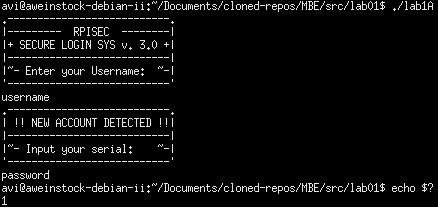
\includegraphics[width=0.9\paperwidth]{pictures/mbe_lab1a_dynamic_fail_cropped.png}
\end{frame}

\begin{frame}[fragile]
\frametitle{MBE Lab1A - Username Entry}
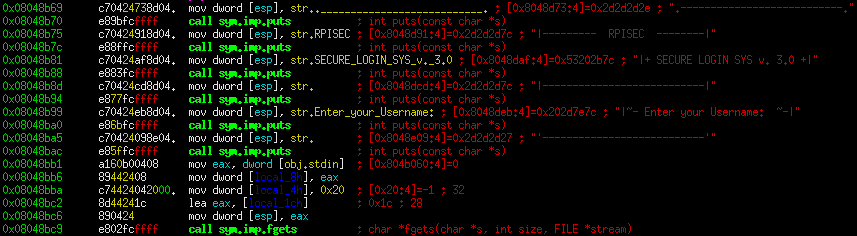
\includegraphics[width=0.9\paperwidth]{pictures/intel/mbe_lab1a_username_entry.png}
\end{frame}

\begin{frame}[fragile]
\frametitle{MBE Lab1A - Serial Entry}
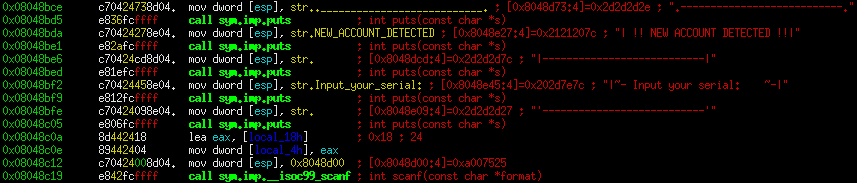
\includegraphics[width=0.9\paperwidth]{pictures/intel/mbe_lab1a_serial_entry.png}\\
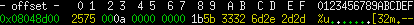
\includegraphics[width=0.9\paperwidth]{pictures/mbe_lab1_scanf_arg_cropped.png}
\end{frame}

\begin{frame}[fragile]
\frametitle{MBE Lab1A - Calling the authentication routine}
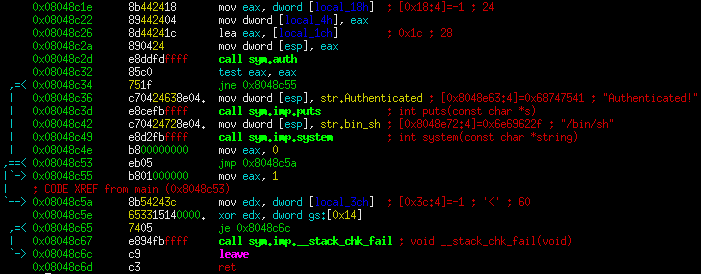
\includegraphics[width=0.9\paperwidth]{pictures/intel/mbe_lab1a_call_auth.png}
\end{frame}

\begin{frame}[fragile]
\frametitle{MBE Lab1A - auth() 1/6: String processing and antidecomp}
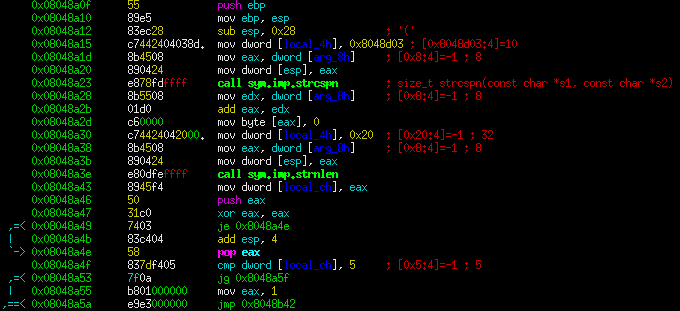
\includegraphics[width=0.9\paperwidth]{pictures/intel/mbe_lab1a_auth_chunk1.png}
\end{frame}

\begin{frame}[fragile]
\frametitle{MBE Lab1A - auth() 2/6: Antidebugging with ptrace}
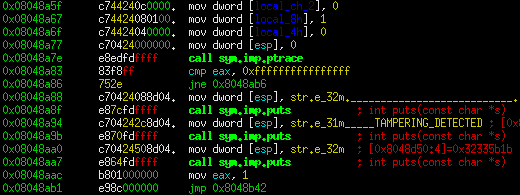
\includegraphics[width=0.9\paperwidth]{pictures/intel/mbe_lab1a_auth_chunk2.png}
\end{frame}

\begin{frame}[fragile]
\frametitle{MBE Lab1A - auth() 3/6: Pre-loop math}
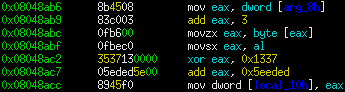
\includegraphics[width=0.9\paperwidth]{pictures/intel/mbe_lab1a_auth_chunk3.png}
\end{frame}

\begin{frame}[fragile]
\frametitle{MBE Lab1A - auth() 4/6: Loop header, restricting chars}
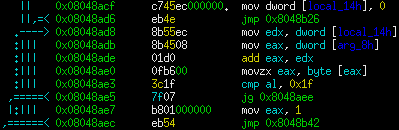
\includegraphics[width=0.9\paperwidth]{pictures/intel/mbe_lab1a_auth_chunk4.png}
\end{frame}

\begin{frame}[fragile]
\frametitle{MBE Lab1A - auth() 5/6: Loop body, much math}
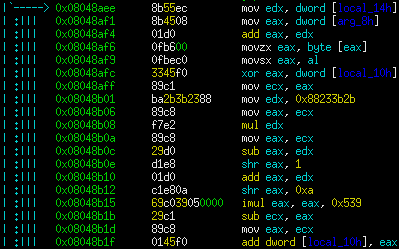
\includegraphics[width=0.8\paperwidth]{pictures/intel/mbe_lab1a_auth_chunk5.png}
\end{frame}

\begin{frame}[fragile]
\frametitle{MBE Lab1A - auth() 6/6: Loop footer, return targets}
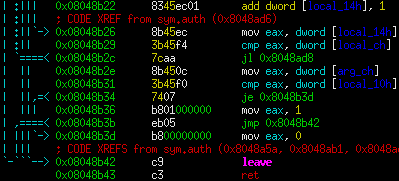
\includegraphics[width=0.9\paperwidth]{pictures/intel/mbe_lab1a_auth_chunk6.png}
\end{frame}

\begin{frame}[fragile]
\frametitle{MBE Lab1A - Z3ing auth() 1/7: Setting up variables}
\begin{Verbatim}[fontsize=\scriptsize, frame=single]
import z3
solver = z3.Solver()
wanted_length = 8
assert wanted_length > 5 # checked at 0x08048a4f
sym_username = [z3.BitVec('x{i}'.format(i=i), 8) for i in range(wanted_length)]
sym_serial = z3.BitVec('serial', 32)
\end{Verbatim}
\begin{itemize}
\item 8-bit entries for each character
\item 32-bit serial number
\item Concrete input length: \verb|z3.Array| exists, but is more expensive
\item Only use \verb|z3.Array| if you need symbolic indexing
\end{itemize}
\end{frame}

\begin{frame}[fragile]
\frametitle{MBE Lab1A - Z3ing auth() 2/7: Translating the pre-loop math}
\begin{Verbatim}[fontsize=\scriptsize, frame=single]
0x08048ab6      8b4508         mov eax, dword [arg_8h]
0x08048ab9      83c003         add eax, 3 ; eax = (arg_8h + 3)
0x08048abc      0fb600         movzx eax, byte [eax] ; eax = *(uint8_t*)(arg_8h+3)
0x08048abf      0fbec0         movsx eax, al ; eax = (int32_t)*(uint8_t*)(arg_8h+3)
0x08048ac2      3537130000     xor eax, 0x1337
0x08048ac7      05eded5e00     add eax, 0x5eeded
0x08048acc      8945f0         mov dword [local_10h], eax
\end{Verbatim}

\begin{Verbatim}[fontsize=\scriptsize, frame=single]
eax = z3.SignExt(24, sym_username[3]) # (int32_t)*((uint8_t*)arg_8h + 3)
eax ^= z3.BitVecVal(0x1337, 32)
eax += z3.BitVecVal(0x5eeded, 32)
local_10h = eax
\end{Verbatim}
\begin{itemize}
\item We're wrapping concrete values in \verb|z3.BitVecVal| so that wrapping/truncation happens the x86 way
\item If we were using python longs here, we'd have to manually mask them back into range
\end{itemize}
\end{frame}

\begin{frame}[fragile]
\frametitle{MBE Lab1A - Z3ing auth() 3/7: Translating the loop header/footer}
The following x86:
\begin{Verbatim}[fontsize=\scriptsize, frame=single]
0x08048acf      c745ec000000.  mov dword [local_14h], 0
0x08048ad6      eb4e           jmp 0x8048b26
...
0x08048b22      8345ec01       add dword [local_14h], 1
0x08048b26      8b45ec         mov eax, dword [local_14h]
0x08048b29      3b45f4         cmp eax, dword [local_ch]
0x08048b2c      7caa           jl 0x8048ad8
\end{Verbatim}
Translates to the following C:
\begin{Verbatim}[fontsize=\scriptsize, frame=single]
for(int local_14h=0; local_14h < local_ch; local_14h++) {
    /* loop body is between 0x08048ad6 and 0x08048b22, exclusive on both ends */
}
\end{Verbatim}
So we'll gloss that as the following in Python
\begin{Verbatim}[fontsize=\scriptsize, frame=single]
local_ch = len(sym_username) # this is set by the strnlen at 0x08048a3e
for local_14h in range(local_ch):
    pass # we'll translate the loop body here
\end{Verbatim}
\end{frame}

\begin{frame}[fragile,t]
\frametitle{MBE Lab1A - Z3ing auth() 4/7: Translating the loop body: 1/2}
\begin{minipage}{0.5\textwidth}x86:\end{minipage}
\begin{minipage}{0.49\textwidth}Python:\end{minipage}
\begin{minipage}{0.5\textwidth}
\begin{Verbatim}[fontsize=\scriptsize, frame=single]
0x08048ad8      mov edx, dword [local_14h]
0x08048adb      mov eax, dword [arg_8h]
0x08048ade      add eax, edx
0x08048ae0      movzx eax, byte [eax]
0x08048ae3      cmp al, 0x1f
0x08048ae5      jg 0x8048aee
\end{Verbatim}
\end{minipage}
\begin{minipage}{0.49\textwidth}
\begin{Verbatim}[fontsize=\scriptsize, frame=single]
solver.add(sym_username[local_14h] > 0x1f)
\end{Verbatim}
\end{minipage}
\begin{minipage}{0.5\textwidth}
\begin{Verbatim}[fontsize=\scriptsize, frame=single]
0x08048aee      mov edx, dword [local_14h]
0x08048af1      mov eax, dword [arg_8h]
0x08048af4      add eax, edx
0x08048af6      movzx eax, byte [eax]
0x08048af9      movsx eax, al
0x08048afc      xor eax, dword [local_10h]
\end{Verbatim}
\end{minipage}
\begin{minipage}{0.49\textwidth}
\begin{Verbatim}[fontsize=\scriptsize, frame=single]
eax = z3.SignExt(24, sym_username[local_14h])
eax ^= local_10h
\end{Verbatim}
\end{minipage}
\begin{minipage}{0.5\textwidth}
\begin{Verbatim}[fontsize=\scriptsize, frame=single]
0x08048aff      mov ecx, eax
0x08048b01      mov edx, 0x88233b2b
0x08048b06      mov eax, ecx
\end{Verbatim}
\end{minipage}
\begin{minipage}{0.49\textwidth}
\begin{Verbatim}[fontsize=\scriptsize, frame=single]
ecx = eax
edx = z3.BitVecVal(0x88233b2b, 32)
eax = ecx
\end{Verbatim}
\end{minipage}
\end{frame}
\begin{frame}[fragile,t]
\frametitle{MBE Lab1A - Z3ing auth() 5/7: Translating the loop body: 2/2}
\begin{minipage}{0.5\textwidth}x86:\end{minipage}
\begin{minipage}{0.49\textwidth}Python:\end{minipage}

\begin{minipage}{0.3\textwidth}
\begin{Verbatim}[fontsize=\scriptsize, frame=single]
0x08048b08      mul edx
\end{Verbatim}
\end{minipage}
\begin{minipage}{0.69\textwidth}
\begin{Verbatim}[fontsize=\scriptsize, frame=single]
mul_result = z3.ZeroExt(32, eax) * z3.ZeroExt(32, edx)
edx = z3.Extract(63, 32, mul_result)
eax = z3.Extract(31, 0, mul_result)
\end{Verbatim}
\end{minipage}
\begin{minipage}{0.5\textwidth}
\begin{Verbatim}[fontsize=\scriptsize, frame=single]
0x08048b0a      mov eax, ecx
0x08048b0c      sub eax, edx
0x08048b0e      shr eax, 1
0x08048b10      add eax, edx
0x08048b12      shr eax, 0xa
\end{Verbatim}
\end{minipage}
\begin{minipage}{0.49\textwidth}
\begin{Verbatim}[fontsize=\scriptsize, frame=single]
eax = ecx
eax -= edx
eax = eax >> 1
eax += edx
eax = eax >> 0xa
\end{Verbatim}
\end{minipage}
\begin{minipage}{0.4\textwidth}
\begin{Verbatim}[fontsize=\scriptsize, frame=single]
0x08048b15      imul eax, eax, 0x539
\end{Verbatim}
\end{minipage}
\begin{minipage}{0.59\textwidth}
\begin{Verbatim}[fontsize=\scriptsize, frame=single]
eax = z3.Extract(31, 0, z3.SignExt(32, eax) * 0x539)
\end{Verbatim}
\end{minipage}
\begin{minipage}{0.5\textwidth}
\begin{Verbatim}[fontsize=\scriptsize, frame=single]
0x08048b1b      sub ecx, eax
0x08048b1d      mov eax, ecx
0x08048b1f      add dword [local_10h], eax
\end{Verbatim}
\end{minipage}
\begin{minipage}{0.49\textwidth}
\begin{Verbatim}[fontsize=\scriptsize, frame=single]
ecx -= eax
eax = ecx
local_10h += eax
\end{Verbatim}
\end{minipage}
\end{frame}

\begin{frame}[fragile]
\frametitle{MBE Lab1A - Z3ing auth() 6/7: Solving for a valid serial}
\begin{Verbatim}[fontsize=\scriptsize, frame=single]
solver.add(sym_serial == local_10h) # outside the loop
solver.push() # backtracking point for next demo
username = 'username'
for (x, y) in zip(username, sym_username):
    solver.add(ord(x) == y)
assert solver.check().r == 1
model = solver.model()
serial = model.evaluate(sym_serial)
print('serial for name %r is %r' % (username, serial))
\end{Verbatim}
\begin{Verbatim}[fontsize=\scriptsize, frame=single]
serial for name 'username' is 6234463
\end{Verbatim}
\end{frame}

%serial for name 'username' is 6234463
%serial for name 'sEa2):2-' is 6234464

\begin{frame}[fragile]
\frametitle{MBE Lab1A - Z3ing auth() 7/7: Solving for a valid username}
\begin{Verbatim}[fontsize=\scriptsize, frame=single]
solver.pop() # remove the constraints on the provided username
solver.add(sym_serial == serial+1)
assert solver.check().r == 1
model = solver.model()
username2 = ''.join(chr(model.evaluate(x).as_long()) for x in sym_username)
serial2 = model.evaluate(sym_serial)
print('serial for name %r is %r' % (username2, serial2))
\end{Verbatim}
\begin{Verbatim}[fontsize=\scriptsize, frame=single]
serial for name 'sEa2):2-' is 6234464
\end{Verbatim}
\end{frame}

\begin{frame}[fragile]
\frametitle{Resources}
\begin{itemize}
\item \verb|https://github.com/Z3Prover/z3/|
\item \verb|https://pypi.org/project/z3-solver/|
\item \verb|https://rise4fun.com/Z3/tutorialcontent/guide|
\item \verb|https://en.wikipedia.org/wiki/Satisfiability_modulo_theories|
\item \verb|https://github.com/RPISEC/MBE|
\end{itemize}
\end{frame}
\end{document}
